En el presente capítulo se expone los métodos utilizados para 
conseguir los objetivos específicos detallados en el Capítulo 
\ref{objetivos}. Cada subsección corresponde con cada uno de 
los objetivos en los que se explicará en qué consiste cada 
objetivo de forma más extendida, la herramienta escogida 
para su realización y la justificación de su elección.

\section{Descripción del \textit{Dataset}}

Para la realización de este trabajo se decidió elegir el 
``\textit{Hockey Fight Detection Dataset}'' el cual es un 
conjunto de datos ampliamente utilizado en la investigación 
sobre detección automática de violencia en videos. Fue 
desarrollado por Enrique Bermejo Nievas, Óscar Deniz Suárez, 
Gloria Bueno García y Rahul Sukthankar, y publicado en 2011 
\cite{nievas2011violence}. 
Este dataset fue concebido para abordar la necesidad de 
sistemas capaces de identificar comportamientos agresivos en 
entornos de vigilancia, como prisiones, centros psiquiátricos 
o residencias de ancianos, donde la detección temprana de 
violencia es crucial.

El conjunto de datos consta de 1,000 secuencias de video, 
divididas equitativamente en dos categorías: 500 videos 
que muestran peleas durante partidos de hockey sobre hielo 
y 500 videos sin violencia. Cada video tiene una duración 
aproximada de 1 a 2 segundos y está etiquetado manualmente 
para facilitar su uso en tareas de clasificación supervisada. 
Los videos fueron recopilados de diversas fuentes, incluidos 
sitios web de noticias y plataformas de video en línea, 
asegurando una variedad de escenarios y condiciones de 
iluminación. En la figura \ref{fig:combinedHockey} se muestra 
una comparación de un frame de cada uno de las etiquetas: 

\begin{figure}[h!]%
    \centering
    \subfloat[\centering Frame conteniendo violencia]{{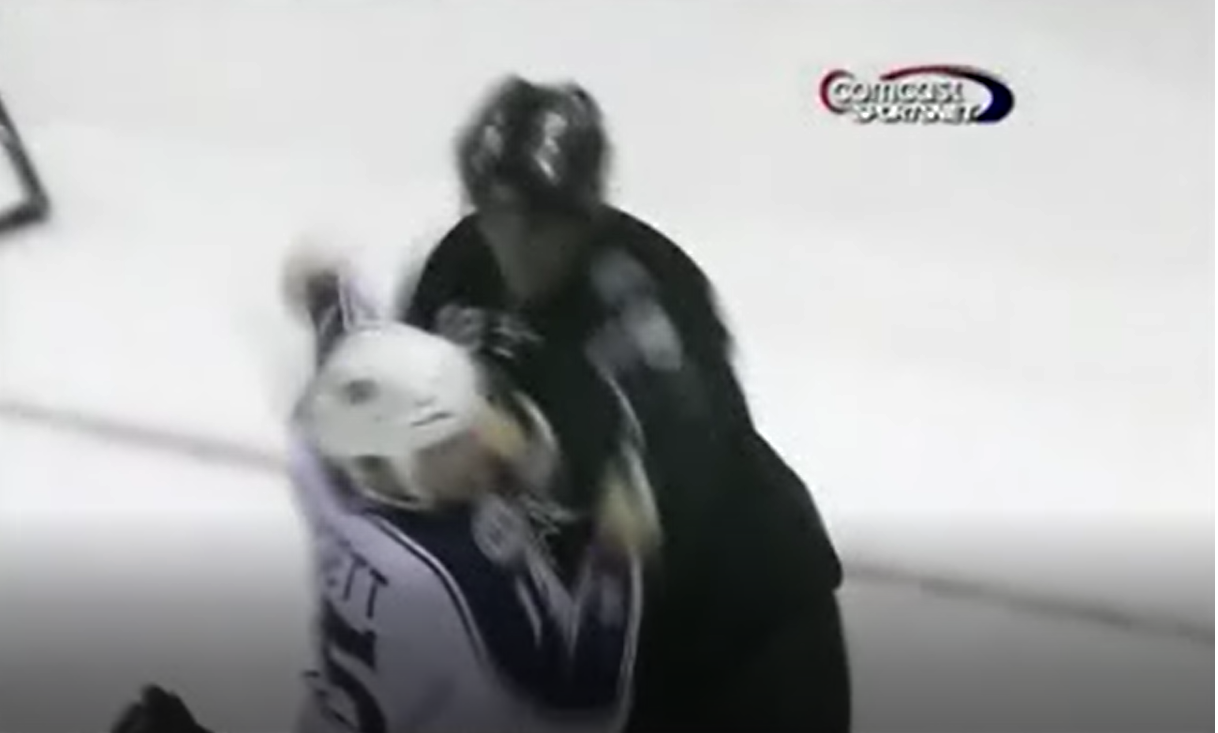
\includegraphics[width=6cm]{images/hockeyFight.png} }}%
    \qquad
    \subfloat[\centering Frame no conteniendo violencia]{{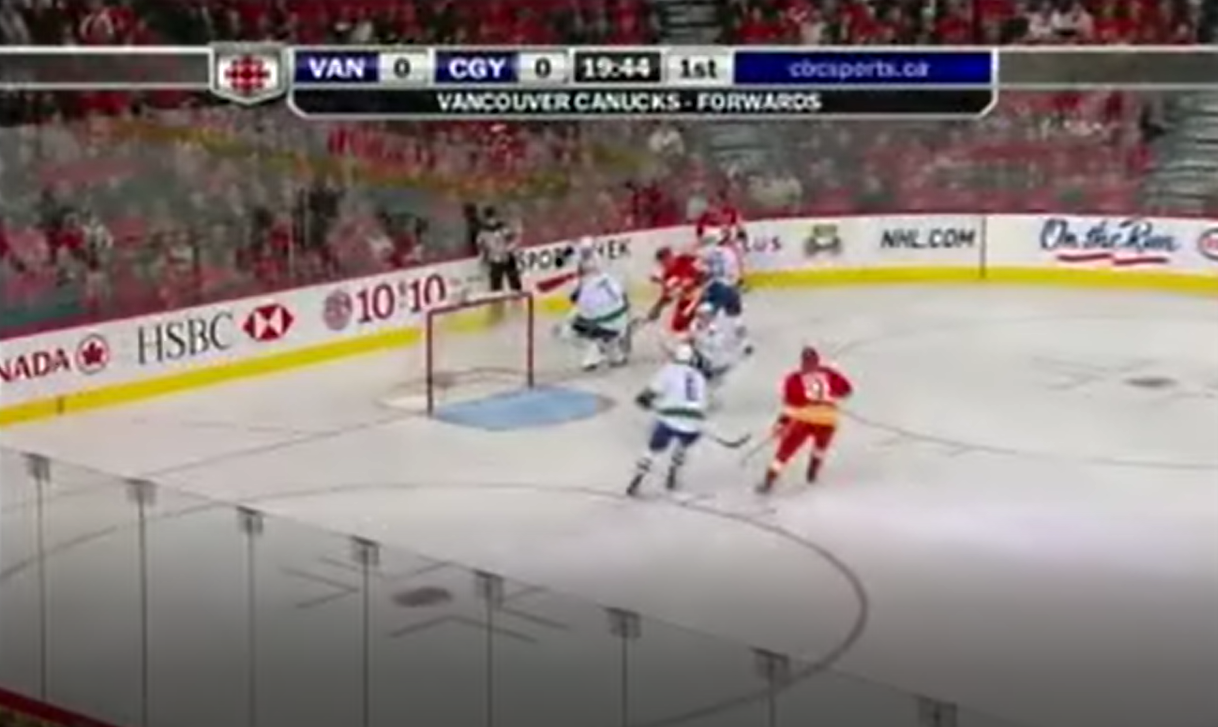
\includegraphics[width=6cm]{images/hockeyNotFight.png} }}%
    \caption{Comparación entre frames con y sin violencia en el ``Hockey Fight Detection Dataset'' }%
    \label{fig:combinedHockey}%
\end{figure}

\section{Pre-procesamiento de la base de datos}

Para preparar los datos del conjunto \textit{Jockey Fights} y 
garantizar su compatibilidad con los modelos de aprendizaje 
profundo utilizados, es necesario el siguiente proceso de 
pre-procesamiento estructurado en varias etapas:

\begin{itemize}
    \item \textbf{Obtención de frames}: Cada video del dataset 
    se descompone en sus respectivos fotogramas (frames) 
    utilizando una frecuencia de muestreo fija. Estos frames 
    fueron almacenados como matrices RGB, representando la 
    información visual en tres canales (rojo, verde y azul), 
    lo cual permitió capturar el contenido visual de cada 
    instante del video.

    \item \textbf{Recorte y redimensionamiento}: Los frames 
    extraídos se redimensionaron a una resolución fija 
    (como 224x224 píxeles), adaptándose así a los 
    requerimientos de entrada de los modelos de red neuronal 
    convolucional (CNN) utilizados en la etapa de extracción 
    de características.

    \item \textbf{Normalización}: Con el objetivo de mejorar 
    la eficiencia del entrenamiento de los modelos, se 
    normalizaron los valores de los píxeles de las imágenes. 
    Esto se realizó escalando los valores del rango [0, 255] 
    al rango [0, 1] o aplicando una normalización estadística 
    basada en la media y desviación estándar de los canales 
    RGB, especialmente útil cuando se emplean modelos 
    preentrenados.

    \item \textbf{Etiquetado de los datos}: A partir de los 
    nombres de los videos y su contexto, se asignaron etiquetas 
    binarias a cada secuencia de imágenes. Los videos fueron 
    clasificados como \textit{violentos} o 
    \textit{no violentos}, y dicha etiqueta fue propagada a 
    todos los frames correspondientes al video, asumiendo 
    homogeneidad del contenido en cada segmento.

    \item \textbf{Filtrado y muestreo}: Para reducir la 
    redundancia y el volumen de datos, se aplicó una 
    estrategia de muestreo temporal, extrayendo únicamente un 
    subconjunto de los frames (por ejemplo, uno de cada cinco). 

\end{itemize}

Este pre-procesamiento es esencial para estandarizar 
los datos, minimizar el ruido y facilitar el posterior 
entrenamiento de los modelos de detección de violencia basados 
en aprendizaje profundo.

\section{Métricas de Evaluación}

Para la evaluación del conjunto de datos 
\textit{Jockey Fights}, se utilizan las siguientes 
métricas de rendimiento:

\begin{itemize}

    \item \textbf{AUC-ROC (Área bajo la curva ROC)}: Evalúa 
    el rendimiento del modelo en todos los umbrales de 
    clasificación posibles. Es útil para modelos binarios, 
    especialmente con clases desbalanceadas.
    
    \item \textbf{Tiempo de Inferencia}: Mide el tiempo que 
    el modelo tarda en procesar una secuencia completa o un 
    solo frame. Es crucial para aplicaciones en tiempo real 
    o streaming.

    \item \textbf{Tiempo de Inferencia}: Mide el tiempo que 
    el modelo tarda en procesar una secuencia completa o un solo frame. Es crucial para aplicaciones en tiempo real o streaming.
\end{itemize}

\section{Software y hardware utilizados}
A lo largo de toda la experimentación, se utilizará un computador de escritorio con las siguientes características:

\begin{table}[h!]
\centering
\footnotesize
\begin{tabular}{|l|l|}
\hline
\textbf{Componente} & \textbf{Descripción} \\ \hline
Procesador & Procesador	Core i5-10300H 2.50GHz\\ \hline
Memoria RAM & 16GB DDR4 - 3600MHZ \\ \hline
Tarjeta Gráfica & Nvidia RTX 3050 4GB \\ \hline
\end{tabular}
\end{table}

Por otra parte, se utilizó Python, junto con Keras, Sklearn y Tensorflow 
para el desarrollo del \textit{pipeline} en general y el pre y post 
procesamiento de los datos. Para el procesamiento de las imágenes (con Yolo) 
se utilizó OpenCV compilado con cudnn para la habilitación del uso de tarjeta gráfica. 
